\documentclass[master=eelt, english]{kulemt}

\setup{
title={Implementation and Evaluation of Zero-Knowledge Proofs of Knowledge},
author={Boran Car},
promotor={Bart Preneel \and Ingrid Verbauwhede},
assessor={Claudia Diaz \and Francky Catthoor},
assistant={Josep Balasch \and Alfredo Rial}
}

\usepackage[pdfusetitle,colorlinks,plainpages=false]{hyperref}
\usepackage{biblatex}
\usepackage{tikz}
\usepackage{tikz-qtree}
\usepackage[caption=false]{subfig}
\usepackage{tabularx}
\usepackage{color}
\usepackage{amsmath}
\usepackage{listings}
\usepackage{amsfonts}
\usepackage{amsthm}
\usepackage{algpseudocode}
\usepackage{algorithm}

\theoremstyle{definition}
\newtheorem{defn}{Definition}
\newtheorem{thm}{Theorem}

\definecolor{dkgreen}{rgb}{0,0.6,0}
\definecolor{gray}{rgb}{0.5,0.5,0.5}
\definecolor{mauve}{rgb}{0.58,0,0.82}

\lstdefinelanguage{PIL}{
morekeywords={ExecutionOrder, Common, Def, Void, Prime, Z, Int},
otherkeywords={Zmod+, Zmod*},
morecomment=[l]{//},
morecomment=[s]{/*}{*/}
}

\lstset{
language=PIL,
basicstyle=\footnotesize,
commentstyle=\color{dkgreen},
keywordstyle=\bfseries,
frame=single,
breaklines=true,
breakatwhitespace=false
}

\usetikzlibrary{backgrounds,calc,shapes,shadows,arrows,chains,trees,fit,positioning}

\tikzstyle{language}=[rectangle,draw=black,thin,inner sep=3pt, align=center]

\tikzstyle{compiler}=[rectangle,rounded corners,draw=black,thin,inner
sep=3pt, align=center]

\tikzstyle{added}=[fill=gray]

\addbibresource{references}

\begin{document}

\begin{preface}

\end{preface}

\tableofcontents*

\begin{abstract}

\end{abstract}

\listoffigures

\listoftables

\mainmatter

%1.1-	Motivation
%- Crypto involves complex building blocks.
%- Among them, ZKPK.
%- Its implementation is complex
%- most programmers are not cryptographers, and thus prone to errors
%- Automated tools for implementing crypto protocols are needed (name some existing tools).
%
%- crypto implementations for embedded devices are demanded
%- new crypto protocols
%- generic tools (GMP, high java level)
%- Existing tools should be adapted to embedded devices.

%In the last years myriad of advanced cryptographic techniques have been proposed and formalized in the open literature. Such protocols go beyond the traditional security goals of data integrity, authentication, and confidentiality, and instead focus on providing other strong security and privacy properties.
%
%Zero-knowledge proofs of knowledge~\cite{Goldwasser:1985:KCI:22145.22178,Goldreich:1987:PNZ:36664.36675,springerlink:10.1007/BF02351717} are amongst the most prominent examples of this trend. These cryptographic tools allow an entity (the \emph{Prover}) to prove knowledge of a statement to another entity (the \emph{Verifier}) without actually revealing any information about such statement. Within a system, ZKPoK can be used to enforce honest behaviour between entities while maintaining their privacy, making such protocols ideal for privacy preserving applications. Just to name a few, zero-knowledge proofs of knowledge are found at the core of systems such as anonymous e-cash~\cite{1982-1101,Camenisch05compacte-cash}, anonymous authentication~\cite{Brickell:2004:DAA:1030083.1030103,Nguyen05dynamick-times}, or electronic voting~\cite{Groth:2005:NZA:2134532.2134564,Damgard03thetheory}.

Zero-knowledge proofs of knowledge (ZKPK)~\cite{Goldwasser:1985:KCI:22145.22178,Goldreich:1987:PNZ:36664.36675,springerlink:10.1007/BF02351717} allow an entity (the \emph{Prover}) to prove knowledge of a secret that fulfills a statement to another entity (the \emph{Verifier}) without revealing any information about the secret. ZKPK can be used as building blocks of cryptographic protocols to enforce the honest behaviour of entities while maintaining their privacy, making such protocols ideal for privacy preserving applications. Just to name a few, ZKPK are found at the core of systems such as anonymous e-cash~\cite{DBLP:conf/crypto/Chaum82,Camenisch05compacte-cash}, anonymous authentication~\cite{Brickell:2004:DAA:1030083.1030103,Nguyen05dynamick-times}, electronic voting~\cite{Groth:2005:NZA:2134532.2134564,Damgard03thetheory} or general secure two-party and multi-party computation~\cite{DBLP:conf/stoc/CanettiLOS02}.

%Such strong security properties come however at a high cost in terms of complexity and efficiency. 

The implementation of ZKPK is error-prone, particularly for programmers not familiar with the underlying cryptographic techniques, which hinders the deployment of protocols that employ ZKPK. To address this problem, there exist nowadays several tools to facilitate ZKPK implementation, either by providing high-level libraries~\cite{Camenisch:2002:DII:586110.586114}, custom made language interpreters and compilers~\cite{Almeida:2010:CCZ:1888881.1888894}, or a mixture of both~\cite{Meiklejohn:2010:ZLS:1929820.1929838}.

Existing tools~\cite{Camenisch:2002:DII:586110.586114,Almeida:2010:CCZ:1888881.1888894,Meiklejohn:2010:ZLS:1929820.1929838} target software (SW) high-level languages such as C, C++ or Java. However, some protocols are naturally expected to be implemented on small embedded platforms, e.g.\ smart cards for storing e-cash wallets, and electronic IDs or TPMs for anonymous authentication~\cite{Brickell:2004:DAA:1030083.1030103}. In such cases, the use of ZKPK compilers that target hardware (HW) description languages and that allow for HW-SW co-design is more convenient.

%While incredibly useful, these tools focus on ZKPoKs as standalone blocks rather than as part of a full application. In other words, there are some limitations such as e.g.\ when implementing systems with multiple participating entities. Similarly, the resulting code is given in high-level languages such as C, C++, or Java, each one using their own cryptographic library, making it difficult to port the code to small embedded devices. This is of importance since, as can be noted from the above mentioned examples, some entities are naturally expected to be implemented on small embedded platforms, e.g.\ smart cards for storing e-cash wallets, electronic IDs or TPMs for anonymous authentication, etc...

%1.2- Our contribution
%- We do not start from scratch
%- We use an existing framework, which we extend and modify
%- Explanation on the main extensions and modifications (why the extension/modification was needed, which functionalities are now possible that were not possible before).
%- Explanation of the new features provided. Focus on all the implementation possibilities (HW languages, embedded devices, HW-SW codesign).
\paragraph{Our contribution.} We provide a ZKPK compiler framework specifically tailored to target hardware description languages and HW-SW co-design. Rather than starting from scratch, we extend the functionalities offered by the CACE ZKPK compiler suite~\cite{Almeida:2010:CCZ:1888881.1888894} to generate platform-independent code and explore hardware/software boundaries. The CACE ZKPK compiler allows the implementation of (the composition of) the most relevant $\Sigma$-protocols, which are the practically relevant ZKPK. 

Concretely, our ZKPK compiler framework follows two steps. First, it takes as input a ZKPK implementation in platform-independent code generated by the CACE ZKPK compiler and transforms it into an implementation in LLVM IR, which is the intermediate representation language of the LLVM compiler framework. The implementation in LLVM IR can be optimized via the LLVM optimizer.

From LLVM IR, it is possible to target different languages. We provide a back-end for GEZEL, a HW description language that can subsequently target VHDL or Verilog, that provides validation tools and that offers a co-simulation tool used for HW-SW co-design purposes. Additionally, we provide a back-end for C, which uses GMP for big integer arithmetic. Therefore, we cover both ends of the HW/SW co-design spectrum.

We consider that our custom ZKPK compiler framework provides a good starting point for a fine-grained automated approach to HW-SW co-design. It  allows the implementation of all the ZKPK supported by the original CACE ZKPK compiler. Additionally, thanks to the characteristics of LLVM IR, we can validate the security of the implementation at a lower level than the one allowed by the CACE ZKPK compiler.

%1.3- Structure of the paper (Explain briefly the contents of each section of the paper)
\paragraph{Structure of the paper.} In Section~\ref{relatedwork} we summarize related work in the area of cryptography aware compilers. In Section~\ref{preliminaries} we provide some background information. The tools used through the paper are briefly introduced in Section~\ref{sec:tools}. Our custom compiler is described in Section~\ref{customframework}, and some discussion topics are addressed in Section~\ref{discussion}. Finally we conclude in Section~\ref{conclusion}.

%%% Local Variables:
%%% TeX-PDF-mode: t
%%% TeX-master: "paper"
%%% End:


\chapter{Technical Preliminaries}

This chapter has the goal of introducing the math and theory behind
formal languages, parsers, algebra, (zero knowledge) proofs of
knowledge, control and data flow in a program. Knowledge behind formal
languages is needed to design a parser which will later on be used to
create a custom compiler framework.

Zero knowledge proofs of knowledge are the basis of this thesis so
they need to be introduced here. First we start with group theory and
modular arithmetic, then we proceed with defining zero knowledge proofs
of knowledge and give a basic example of a protocol.

We conclude the chapter with introducing control flow graphs and data
flow (data dependency) graphs which are needed to reason about the
intermediate form the compiler generates.

\section{Formal Languages}

The theory of formal languages is needed to introduce a parser which
is the basic building block of a compiler. Here we give a short
overview of formal languages based on \cite{formal_languages} and for
a more detailed approach refer the reader to \cite{Hopcroft}.

We start with basic definitions of a formal language:

\begin{defn}[Alphabet]
  An alphabet $\Sigma$ is a set of symbols.
\end{defn}

\begin{defn}[String]
  A string over an alphabet $\Sigma$ is a sequence of symbols of $\Sigma$.
\end{defn}

\begin{defn}[Concatenation]
  Let $x = a_0 a_1 \dotsm a_n$ and $y = b_0 b_1 \dotsm b_n$, then the
  string $x y = a_0 a_1 \dotsm a_n b_0 b_1 \dotsm b_n$ is the
  concatenation of the strings $x$ and $y$.
\end{defn}

\begin{defn}[Sets]
  $\Sigma^*$ denotes the set of all the strings over the alphabet
  $\Sigma$. Likewise, $\Sigma^+$ denotes the set of all the non-empty
  strings over the alphabet $\Sigma$. $$\Sigma^+ \subseteq \Sigma^*
  \setminus \{ \epsilon \}$$ The empty set of strings is denoted
  $\emptyset$.
\end{defn}

\begin{defn}[Language]
  A language over the alphabet $\Sigma$ is a set of strings over
  $\Sigma$. Members of the language are called words of the language.
\end{defn}

\begin{defn}[Concatenation]
  Let $L_1$ and $L_2$ be two languages over alphabet $\Sigma$, the
  language $L_1 L_2 = \{x y | x \in L_1, y \in L_2 \}$ is the
  concatenation of $L_1$ and $L_2$.
\end{defn}

\begin{defn}[Kleene closure]
  Let $L$ be a language over $\Sigma$. Define 
  $$L^0 = \{ \epsilon \}$$
  $$L^i = L L^{i-1} \; \textrm{for} \; i \ge 1$$
  The \emph{Kleene closure} of $L$, denoted by $L^*$, is the language:
  $$ L^* = \bigcup_{i \ge 0} L^i $$
  the \emph{positive closure} is
  $$ L^+ = \bigcup_{i \ge 1} L^i $$
  It can be observed that
  $$ L^* = L^+ \cup \{ \epsilon \} $$
  $$ L^+ = L L^* $$
\end{defn}

We now have a formal basis to define a more powerful tool called
regular expressions. These regular expressions will allow us to
formally, yet compactly, specify the words of a language.

\subsection{Regular Expression}

When writing lexer rules for our compiler, we will need a language
that defines words of the language of our interest. Such a language is
called regular expressions and we briefly define it here:

\begin{defn}[Regular expression]
  A regular expression over $\Sigma$ is defined inductively as follows:
  \begin{enumerate}
  \item $\emptyset$ is a regular expression and represents the empty language
  \item $\epsilon$ is a regular expression and represents the language
    $L = \{ \epsilon \}$
  \item For each $c \in \Sigma$, $c$ is a regular expression and
    represents the language $L = \{ c \}$
  \item For any regular expressions $r$ of language $R$ and $s$ of language $S$:
    \begin{itemize}
    \item $r+s$ is a regular expression representing language $R \cup S$
    \item $r s$ is a regular expression representing language $R S$
    \item $r^*$ is a regular expression representing language $R^*$
    \item $r^+$ is a regular expression representing language $R^+$
    \end{itemize}
  \end{enumerate}
\end{defn}

\begin{thm}
  $r r^*$ can be represented as $r+$
\end{thm}

\begin{proof}
  $r r^*$ represents the language $R R^*$ which is $R^+$
\end{proof}

Now that we have the tool to specify the words of our language, we
need to specify the interactions between these words (e.g. which words
can follow a certain word, what the word ordering is). Such rules are
specified by grammars.

\subsection{Grammars}

When writing parser rules, we will need a language to specify the
interactions between the words of our language. Such a language
is called a grammar and we briefly define it here:

\begin{defn}[Grammar]
  A grammar is a 4-tuple $G = \left< \Sigma, V, S, P \right>$:
  \begin{enumerate}
  \item $\Sigma$ is a finite non-empty set called the \emph{terminal
    alphabet}. The elements of $\Sigma$ are called \emph{terminals}.
  \item $V$ is a finite non-empty set disjoint from $\Sigma$. The
    elements of $V$ are called \emph{non-terminals} or \emph{variables}.
  \item $S \in V$ is a distinguished symbol called the \emph{start symbol}
  \item $P$ is a finite set of \emph{productions (rules)} of the form
    $$ \alpha \rightarrow \beta $$
    $$ \alpha \in (\Sigma \cup V)^* V (\Sigma \cup V)^* $$
    $$ \beta \in (\Sigma \cup V)^* $$
  \end{enumerate}
\end{defn}

\begin{defn}[Context-free grammar]
  The grammar $G$ is a context free grammar iff $|\alpha|$ = 1 ($\alpha = V$).
\end{defn}

We now have all the tools to specify the input language of our
compiler. The parser of our compiler will transform an input file,
according to these rules, to a form suitable for further
processing. The forms we deal at this step are concrete syntax trees
and abstract syntax trees.

\subsection{Concrete Syntax Tree}

A Concrete Syntax Tree, also called a Parse Tree, is an ordered tree
representation of the input according to a given formal grammar.

For example, given the following input:
\begin{lstlisting}
a := b * c + d;
\end{lstlisting}
and the following grammar:
\begin{align*}
  \textrm{statement}  & \rightarrow \textrm{ID} := \textrm{expression} ; \\
  \textrm{expression} & \rightarrow \textrm{term} + \textrm{term} \\
  \textrm{term}       & \rightarrow \textrm{ID} * \textrm{ID} \\
  \textrm{term}       & \rightarrow \textrm{ID}
\end{align*}
the tree depicted in Figure \ref{fig:simple_cst} is a Concrete Syntax Tree.

\begin{figure}[hbt!]
  \centering
  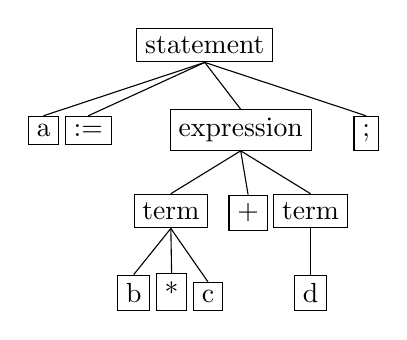
\begin{tikzpicture}
    \Tree [.\node[language](statement){statement};
      [.\node[language](a){a};]
      [.\node[language](assign){:=};]
      [.\node[language](expression){expression};
        [.\node[language](term){term};
          [.\node[language](b){b};]
          [.\node[language](mul){*}; ]
          [.\node[language](c){c};]
        ]
        [.\node[language](plus){+};]
        [.\node[language](term2){term};
          [.\node[language](d){d};]
        ]
      ]
      [.\node[language](semi){;};]
    ]
  \end{tikzpicture}
  \caption{Concrete Syntax tree for a simple input and a simple grammar}
  \label{fig:simple_cst}
\end{figure}

\subsection{Abstract Syntax Tree}

An Abstract Syntax Tree (AST) is a tree representation of the abstract
syntax of the input. Given the same example
\begin{lstlisting}
a := b * c + d;
\end{lstlisting}
one possible variant of the tree is illustrated in Figure
\ref{fig:simple_ast}. Comparing it with the Parse Tree from Figure
\ref{fig:simple_cst} one can see that the choice of abstraction is
arbitrary.

\begin{figure}[hbt!]
  \centering
  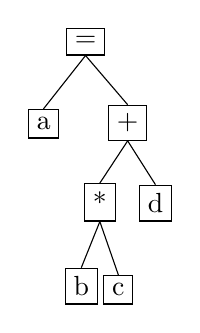
\begin{tikzpicture}
    \Tree [.\node[language](equ){=};
      [.\node[language](a){a};]
      [.\node[language](add){+};
        [.\node[language](mul){*};
          [.\node[language](b){b};]
          [.\node[language](c){c};]
        ]
        [.\node[language](d){d};]
      ]
    ]
  \end{tikzpicture}
  \caption{An example AST for a simple expression}
  \label{fig:simple_ast}
\end{figure}

After all the definitions of the input and the output have been made,
it remains to define the actual tool transforming from the input to
the output. This tool is referred to as the parser.

\subsection{Parser}

Given a string $L$, satisfying grammar $G$, a parser tries to find the
derivation of $L$ from $S$. This derivation is the Concrete Syntax
Tree (Parse Tree). This derivation may further be abstracted into an
Abstract Syntax Tree that is easier for later manipulation. Figure
\ref{fig:parser_flow} shows the typical parser flow.

\begin{figure}[hbt!]
  \centering
  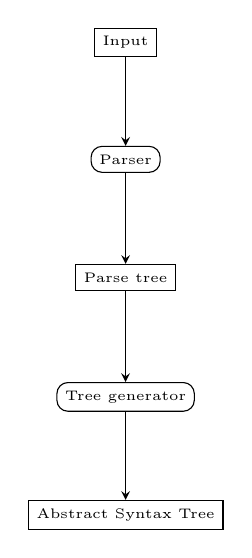
\begin{tikzpicture}[>=stealth,level distance=1.5cm,font=\tiny]
    \tikzstyle{edge from parent}=[draw,->]

    \Tree [.\node[language](input){Input};
      [.\node[compiler](parser){Parser};
        [.\node[language](ptree){Parse tree};
          [.\node[compiler](tgen){Tree generator};
            [.\node[language](ast){Abstract Syntax Tree};
            ]
          ]
        ]
      ]
    ]
  \end{tikzpicture}
  \caption{Parser flow}
  \label{fig:parser_flow}
\end{figure}

There are two approaches to parsing:
\begin{description}
\item[Top-down parsing] the derivation starts from the top (the root)
  of the parse tree and proceeds downwards.
\item[Bottom-up parsing] the derivation starts from the bottom (the
  leaves) of the parse tree and proceeds upwards.
\end{description}

The most popular top-down parser is an LL (left to right left-most
derivation) parser. The parser reads the input left to right and at
each step produces the left-most derivation of the input. Sub-types of
this parser include the symbol look-ahead which is the amount of next,
unseen symbols the parser can ``look at''. For example, an LL(1)
parser can only look 1 symbol ahead while an LL(*) parser is a parser
with arbitrary look-ahead.

\section{Group Theory and Modular Arithmetic}

Before we go into defining proofs of knowledge we need to define the
space we are operating on. We base our definitions on \cite{HAC}, but
the approach we take is a bit different. We choose to start with the
general and deduce the specific from it rather than taking an
inductive approach.

\begin{defn}[Group]
  A group $(G, \circ)$ is a set G with a binary operation $\circ$ defined on it
  that satisfies the following properties:
  \begin{enumerate}
  \item (Closure) $a, b \in G \implies a \circ b \in G$ 
  \item (Associativity) $(a \circ b) \circ c = a \circ (b \circ c)$ $\forall a,b,c \in G$
  \item (Identity element) $\exists I \in G$ such that $a \circ I = I \circ a = a$
  \item (Inverse element) ($\forall a \in G)(\exists a^{-1} \in G)$ such that $a \circ
    a^{-1} = a^{-1} \circ a = I$
  \end{enumerate}
\end{defn}

\begin{defn}[Abelian Group]
  A group $G$ is abelian iff $a \circ b = b \circ a$ $\forall a,b \in G$
\end{defn}

\begin{defn}[Finiteness and Order]
  A group $G$ is finite iff $|G|$ is finite. The number of elements in
  $G$ is called the \emph{order} of the group.
\end{defn}

\begin{defn}[Subgroup]
  A non-empty subset $H \subseteq G$ is a subgroup iff $H$ itself is a
  group w.r.t. to the binary operation of $G$. $H$ is a proper subgroup
  iff $H \neq G$.
\end{defn}

\begin{defn}[Cyclic Group]
  A group $G$ is cyclic iff $(\exists a \in G)(\forall b \in G)(i is
  Integer | b = a^i)$. Such an $a$ is called a generator of $G$. The
  group generated by $a$ is denoted as $\left< a \right>$.
\end{defn}

\begin{defn}[Order]
  Let $G$ be a group and $a \in G$. The order of $a$ is the least
  positive integer $t$ such that $a^t = I$, provided that such an
  integer exists.  If such an integer does not exist, the order is
  defined to be $\infty$.
\end{defn}

\begin{thm}[Lagrange's Theorem]
  If $G$ is a finite group and $H$ is a subgroup of $G$ then $|H|$ divides
  $|G|$.
\end{thm}

\begin{corr}
  The order of $a \in G$ divides $|G|$.
\end{corr}

\begin{defn}[Congruency]
  An integer $a$ is said to be congruent to integer $b$ modulo integer
  $n$, written $a \equiv b \pmod{n}$, iff $n$ divides $a-b$ (denoted as
  $n | a - b$). $n$ is called the \emph{modulus} of the congruency.
\end{defn}

\begin{defn}[Greatest Common Divisor]
  Given two integers $a$ and $b$, the greatest common divisor
  $d=\gcd(a,b)$ is the largest integer $d$ such that $d | a$ and $d | b$.
\end{defn}

\begin{defn}
  Two integers, $a$ and $b$, are relatively prime to each other iff
  \mbox{$\gcd(a,b)=1$}.
\end{defn}

\begin{defn}
  The integers modulo $n$, denoted $Z_n$, is the set of integers
  \mbox{$\{ 0,1,2,\ldots,n-1 \}$}.
\end{defn}

\begin{thm}
  Let $d = \gcd(a, n)$. Then the congruence equation $a x = b \pmod{n}$ has
  $d$ solutions $x$ iff $d$ divides $b$.
\end{thm}

\begin{corr}
  Let $a \in Z_n$. $a$ has a multiplicative inverse, denoted $a^{-1}$,
  iff \mbox{$\gcd(a, n) = 1$}.
\end{corr}

\begin{defn}
  The multiplicative group of $Z_n$ is $Z_n^* = \{a | \gcd(a,n) = 1
  \}$.  Specifically, if $n$ is prime, $Z_n^* = \{a | 1 \leq a \leq n-1
  \}$. The identity element of the multiplicative group is $1$.
\end{defn}

\begin{defn}
  The additive group of $Z_n$ is $Z_n^+ = \{a | 0 \leq a \leq n-1 \}$.
\end{defn}

\begin{defn}[Euler Phi Function]
  The Euler phi function, $\phi(n)$, also called Euler totient
  function, gives the number of integers from the interval $[1,n]$
  which are relatively prime to $n$.
\end{defn}

\begin{corr}
  The order of the group $Z_n^*$ is $\phi(n)$.
\end{corr}

\begin{corr}
  For a prime $p$, $\phi(p) = p-1$.
\end{corr}

\begin{corr}
  If $\gcd(m, n) = 1$, $\phi(m n) = \phi(m) \phi(n)$.
\end{corr}

\begin{thm}[Euler's Theorem]
  If $a \in Z_n^*$, then $a^{\phi(n)} = 1 \pmod{n}$.
\end{thm}

\begin{corr}[Fermat's Theorem]
  If $a \in Z_p^*$, where $p$ is prime, then $a^{p-1} = 1 \pmod{p}$.  
\end{corr}

\begin{corr}
  $a \in Z_n^*$ is a generator of the group $Z_n^*$ iff the order of
  $a$ is $\phi(n)$. $a$ is also called a primitive element of $Z_n^*$
  then.
\end{corr}

After defining the space we are operating on, it remains to define the
basis of this thesis, zero knowledge proofs of knowledge.

\section{Zero Knowledge Proofs of Knowledge}

Zero knowledge proofs of knowledge give us a powerful tool that allows
us to prove knowledge of a secret without actually revealing the
secret.  Here we need a more formal definition which we take from
\cite{Cameni98} and present as a brief overview. Some minor additions
were added for clarity.

\begin{defn}[Interactive Proof of Knowledge]
  Let $R \subseteq \{0,1\}^* \times \{0,1\}^*$ be a polinomially
  bounded binary relation and let $L_R$ be the language defined by
  $R$. An interactive proof of knowledge is a protocol $(P, V)$ that
  has the following properties:
  \begin{enumerate}
  \item (Completeness) $(x,w) \in R \implies [V, P(w)](x) = T$
  \item (Validity) There exists a probabilistic expected polynomial-time
    machine $K$ (Knowledge extractor) such that for every $\tilde{P}$, for
    all polynomials $f(\cdot)$ and all sufficiently large $x \in L_R$:
    \[
    p((x, K^{\tilde{P}(x)}) \in R) \geq p([V, \tilde{P}](x) = T) -
    \frac{1}{f(|x|)}
    \]
    The probabilities are taken over all random choices of $V$, $P$,
    $\tilde{P}$, $K$. The notation $\left[V, P(w)\right](x)$ denotes
    the protocol execution with the secret $x$ and the prover output
    $w$. $\tilde{P}$ includes malicious provers. $K^{\tilde{P}(x)}$
    denotes oracle access to $\tilde{P}(x)$. $f(\cdot)$ denotes the
    knowledge error.
  \end{enumerate}
\end{defn}

\begin{defn}[Soundness] $(\forall \tilde{P})(\forall x \notin
  L_R)(p([V, \tilde{P}](x) = T) < \frac{1}{2})$
\end{defn}
The additional soundness property is associated with $x \notin L_R$.  By
repeating the protocol many times, it can be made arbitrarily small
\cite{Cameni98}.

\begin{defn}[Indistinguishability]
  Let $L \in \{0,1\}^*$ be a language and let $A = \{A(x)\}_{x \in L}$
  and $B = \{B(x)\}_{x \in L}$ be two ensembles of random variables
  indexed by $L$. Ensembles $A$ and $B$ are:
  \begin{itemize}
  \item perfectly indistinguishable if for all $x \in L$ the variables
    $A(x)$ and $B(x)$ are identically distributed
  \item statistically indistinguishable if for every polynomial $f()$
    and for all sufficiently long $x \in L$:
    \[
    \sum_{\alpha \in \{0,1\}^*} | p(A(x) = \alpha) - p(B(x) = \alpha)|
    < \frac{1}{f(|x|)}
    \]
  \item computationally indistinguishable if for every probabilistic
    polynomial-time algorithm $D$, for every polynomial $f()$ and for
    all sufficiently long $x \in L$:
    \[
    |p(D(x, A(x) = 1) - p(D(x, B(x) = 1)| < \frac{1}{f(|x|)}
    \]
  \end{itemize}
\end{defn}

\begin{defn}[Zero-Knowledge]
  An interactive protocol $(P, V)$ is said to be
  perfectly/statistically/computationally zero-knowledge if for
  every probabilistic polynomial-time verifier $\tilde{V}$ there
  exists a probabilistic expected polynomial time simulator
  $S_{\tilde{V}}$ so that the two ensembles
  \[
  \{[\tilde{V}, P(w)](x)\}_{x \in L} \; \textrm{and} \; \{S_{\tilde{V}}(x)\}
  \]
  are perfectly/statistically/computationally indistinguishable.
\end{defn}

\begin{defn}[Honest Verifier Zero-Knowledge]
  An interactive protocol $(P, V)$ is said to be
  perfectly/statistically/computationally zero-knowledge if there
  exists a probabilistic expected polynomial time simulator
  $S_{\tilde{V}}$ so that the two ensembles
  \[
  \{[V, P(w)](x)\}_{x \in L} \; \textrm{and} \; \{S_V(x)\}
  \]
  are perfectly/statistically/computationally indistinguishable.
\end{defn}

To make a more practical definition we restrict to a subset of zero
knowledge proofs of knowledge called $\Sigma$-protocols.

\subsection{$\Sigma$-protocols}

A $\Sigma$-protocol is a three round honest verifier zero-knowledge
proof of knowledge \cite{cryptography_introduction}. The name comes
from the protocol's flow resemblance to the Greek letter $\Sigma$ as
shown in Figure \ref{fig:sigma_flow}. The rounds of the protocol are:
\begin{enumerate}
\item Commitment ($t$) - the prover commits to a value and sends that
  value to the verifier
\item Challenge ($c$) - the verifier computes a random challenge and asks
  the prover to output a value for that challenge
\item Response ($s$) - the prover responds with a new computed value
\end{enumerate}

\begin{figure}[h]
  \centering
  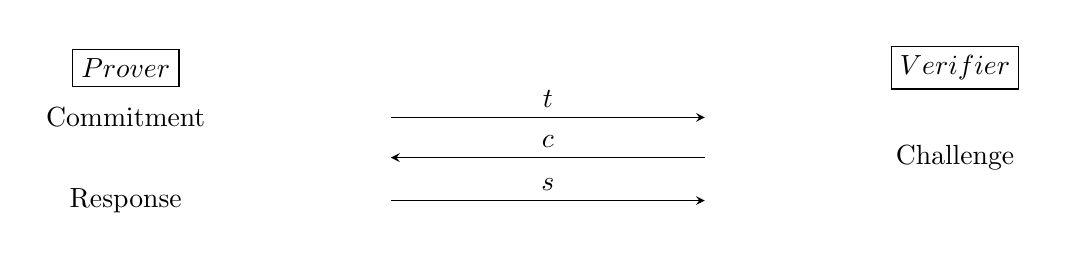
\begin{tikzpicture}[>=stealth]
    \node[matrix,column sep=2cm] {
      \node{\boxed{Prover}};                  &                           & &                             & \node{\boxed{Verifier}}; \\
      \node{Commitment};          & \node(commitment_s){}; & & \node(commitment_r){}; & \\
                                      & \node(challenge_r){}; & & \node(challenge_s){}; & \node{Challenge}; \\
      \node{Response}; & \node(response_s){}; & & \node(response_r){}; & \\
    };
    \draw[->] (commitment_s) -- (commitment_r) node[midway, anchor=south]{$t$};
    \draw[<-] (challenge_r) -- (challenge_s) node[midway, anchor=south]{$c$};
    \draw[->] (response_s) -- (response_r) node[midway, anchor=south]{$s$};
  \end{tikzpicture}
  \caption{Sigma protocol flow}
  \label{fig:sigma_flow}
\end{figure}

\subsubsection{Schnorr's Identification Protocol}
\label{subsubsec:schnorr_protocol}

A simple example of a $\Sigma$ protocol is Schnorr's Identification
Protocol \cite{schnorr_protocol, cryptography_introduction}. The
secret is a discrete logarithm $x$ of $y$ with respect to $g$ in some
finite group $G = \left< g \right>$ with prime order $q$, subgroup of
$Z_p^*$. The prover must prove knowledge of this secret to a verifier
under the homomorphism $f(a) : Z_q^+ \rightarrow G \subset Z_p^* :=
g^a$. Figure \ref{fig:schnorr_steps} gives an overview of the protocol
execution.

\begin{figure}[h]
  \centering
  \begin{tikzpicture}[>=stealth]
    \node[matrix,column sep=2cm] {
      \node{\boxed{Prover}};                  &                           & &                             & \node{\boxed{Verifier}}; \\
      \node{$r_1 \in Z_q^+$};                   &                           & &                             &                   \\
      \node{$t_1 = g^{r_1}$};          & \node(prover_round1_s){}; & & \node(verifier_round1_r){}; & \\
                                      & \node(prover_round2_r){}; & & \node(verifier_round1_s){}; & \node{$c \in \{0,1\}^*$}; \\
      \node{$s_1 = r_1 + x \cdot c$}; & \node(prover_round2_s){}; & & \node(verifier_round2_r){}; & \\
                                      &                           & &                             & \node{$s_1 \stackrel{?}{\in} Z_q^+$}; \\
                                      &                           & &                             & \node{$t_1 y^c \stackrel{?}{=} g^{s_1}$}; \\
    };
    \draw[->] (prover_round1_s) -- (verifier_round1_r) node[midway, anchor=south]{$t_1$};
    \draw[<-] (prover_round2_r) -- (verifier_round1_s) node[midway, anchor=south]{$c$};
    \draw[->] (prover_round2_s) -- (verifier_round2_r) node[midway, anchor=south]{$s_1$};
  \end{tikzpicture}
  \caption{Schnorr's Identification Protocol}
  \label{fig:schnorr_steps}
\end{figure}

\subsubsection{Camenisch-Stadler Notation}
\label{subsubsec:camenisch_stadler}

A simple and popular notation for specifying Sigma protocols is the
Camenisch-Stadler notation \cite{camenisch_stadler}. The Schnorr
Identification Protocol can be represented by the following:
\[
  \textrm{ZPK}\left[ (x): y = g^x \right]
\]
meaning prove knowledge of $x$, using a zero knowledge proof of
knowledge, such that $y=g^x$.

\filbreak

\section{Data Flow Graph and Control Flow Graph}

Our compiler will generate an intermediate form used for detailed
processing. This form is supposed to represent all the operations of
the protocol and can be represented as a directed graph detailing the
flow of the program.

The protocol is input via a text-file and is inherently
sequential. This means that the operations are laid out one after the
other. This inherently imposed ordering need not be the only one and
to make a better ordering w.r.t. to some goal we need constructs that
will allow us to extract all the constraints on the ordering. We keep
the nodes representing the operations while we classify each of the
edges as either a Data Edge or a Control Edge:
\begin{defn}[Data Edge]
  A data edge is an ordered relation between two operations such that
  the output/result of one operation is the input to the other.
\end{defn}
\begin{defn}[Control Edge]
  A control edge is an ordered relation between two operations such
  that the second operation has to be executed after the first finishes
  executing.
\end{defn}

The resulting graph can be separated into two independent graphs called
a Data Flow Graph and a Control Flow Graph.

\begin{defn}[Data Flow Graph]
  A data flow graph is a graph of the nodes representing the
  operations connected by data edges.
\end{defn}

\begin{defn}
  A control flow graph is a graph of the nodes representing the
  operations connected by control edges.
\end{defn}

A Data Flow Graph (DFG) completely and uniquely specifies the
algorithm, whereas the Control Flow Graph (CFG) gives the actual
implementation of the algorithm. After extracting the DFG, a different
CFG can be constructed satisfying the constraints of the
DFG~\cite{Schaumont}.

%%% Local Variables: 
%%% TeX-PDF-mode: t
%%% TeX-master: "thesis"
%%% End: 


\chapter{Existing Frameworks and Tools}

This chapter starts with an overview of existing frameworks for
implementing Zero Knowledge Proofs of Knowledge. Current examples
include CACE Project Zero Knowledge Compiler, ZKPDL and IBM
Idemix. CACE project will be covered in more detail while ZKPDL will
be briefly mentioned. The chapter then continues on describing other
tools that will be used for this thesis: ANTLR, a parser generator
tool producing LL(*) parsers and LLVM, a compiler infrastructure
framework that has seen wide use recently in many fields relating to
compilers and computers in general. ANTLR and LLVM will be used to
make a custom compiler so some knowledge about them is necessary. Next
is GEZEL, a cycle-true cosimulation environment which can also
generate VHDL or Verilog.

\section{CACE Project}

\subsection{Framework Overview}

The CACE (Computer Aided Cryptography Engineering)
Project\footnote{http://www.cace-project.eu} was an European project
aiming at developing a toolbox for security software. It attempted to
ease the creation of cryptographic software for those outside the
domain. The goals were:
\begin{itemize}
\item Automatic translation from natural specification - the
  term natural is taken from the user's perspective, meaning something
  ``natural'' for the user, not dwelling too much into the specific
  niches of cryptography, giving an abstract overview
\item Automatic security awareness, analysis and corrections - to be
  able to detect side channels that are unintentionally introduced,
  warn the user and offer corrective actions
\item Automatic optimization for diverse platforms - different
  platforms are suited for different operations, assume different
  usage patterns etc\ldots, the toolbox should be as most insensitive
  as it can to the platform it is implemented on
\end{itemize}

Apart from these goals that deal with the end-user, the project had
strategic goals of opening a new field of research and promoting
automatic tools when it comes to crypto software. The project itself
was split into multiple working groups:
\begin{itemize}
\item WP1 Automating Cryptographic Implementation - dealing with the
  low level crypto operations, searching and identifying side channel
  attacks, providing a domain specific language
\item WP2 Accelerating Secure Network - dealing with basic operations
  for module intercommunication
\item WP3 Bringing Proofs of Knowledge to Practice - dealing with
  implementing a compiler for Proofs of Knowledge
\item WP4 Securing Distributed Management of Information - dealing
  with higher operations for module intercommunication
\item WP5 Formal Verification and Validation - dealing with analysis
  of the correctness, assuring the user of the protocol validity
\end{itemize}

The WP3 working group is of the importance for this thesis as it deals
directly with proofs of knowledge. The end result of the working group
was a compiler along with a specification language (PSL) and an
intermediate language (PIL). The compiler has the following typical
flow (as depicted in Figure \ref{fig:cace_workflow}):
\begin{enumerate}
\item Write PSL (Protocol Specification Language) - the user specifies the
  protocol using Camenisch-Stadler notation (see Sub-subsection
  \ref{subsubsec:camenisch_stadler})
\item Generate PIL (Protocol Interface Language) from PSL - the
  framework transform it into a lower-level language for specifying
  operations
\item Generate C or Java code from PIL - the framework generates a
  code that is possible to compile and execute on a target
  architecture
\item (Optional) Verify PIL code using PVT - the framework applies the
  formal verification to the PIL code
\item (Optional) Generate LaTeX from PIL - the framework generates
  \LaTeX code with the protocol flow
\end{enumerate}

\begin{figure}[hb!]
  \centering
  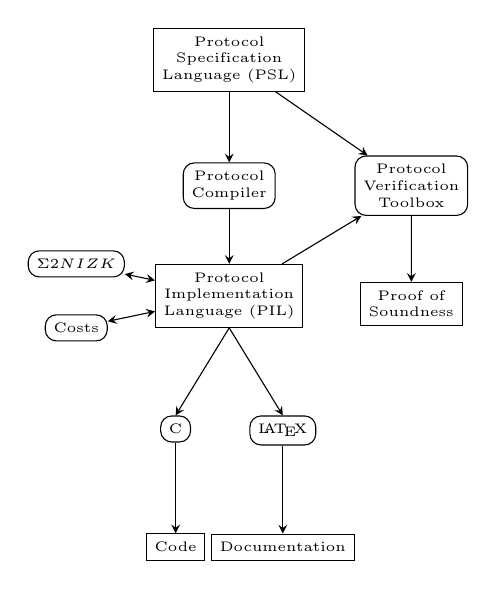
\begin{tikzpicture}[>=stealth,level distance=1.5cm,font=\tiny]
    \tikzstyle{edge from parent}=[draw,->]

    \Tree [.\node[language](psl){Protocol \\ Specification \\ Language (PSL)};
      [.\node[compiler](pc){Protocol \\ Compiler};
        [.\node[language](pil){Protocol \\ Implementation \\ Language (PIL)};
          [.\node[compiler](c){C}; \node[language](code){Code};]
          [.\node[compiler](latex){\LaTeX}; \node[language](doc){Documentation};]
        ]
      ]
    ]

    \node[compiler] (pvt)         [right=of pc,anchor=west]          {Protocol \\ Verification \\ Toolbox}
    child {node[language] {Proof of \\ Soundness}};

    \node[compiler] (sigma) [left=of pil.north west,anchor=center] {$\Sigma 2 N I Z K$};
    \node[compiler] (cost) [left=of pil.south west,anchor=center] {Costs};

    \draw[<->] (sigma) -- (pil);
    \draw[<->] (cost) -- (pil);

    \draw[->] (psl) -- (pvt);
    \draw[->] (pil) -- (pvt);
  \end{tikzpicture}
  \caption{CACE Project Zero Knowledge Compiler typical workflow \cite{CACE}}
  \label{fig:cace_workflow}
\end{figure}

\subsection{PSL}
\label{subsec:psl}

The Protocol Specification Language (PSL) is a high level language of
CACE Project WP3 for specifying Proofs of Knowledge based on
Camenisch-Stadler notation. It allows specification of complex
$\Sigma$ protocols \cite{CACE, yaczk}. The explanation is best given
following an example of a simple protocol, Schnorr's Identification
Protocol (see Sub-subsection \ref{subsubsec:schnorr_protocol}). The
Camenisch-Stadler notation is:
\[
  \textrm{ZPK}\left[ (x): y = g^x \right]
\]

The PSL language is structured into blocks, and for the Schnorr
example the blocks are as follows:
\begin{itemize}
\item Declarations - specifying all the variables used within
  the protocol
\begin{lstlisting}[language=PSL]
Declarations {
  Prime(1024) p;
  Prime(160) q;
  Zmod+(q) x;
  Zmod*(p) g, y;
}
\end{lstlisting}
  This example shows how to declare prime numbers as well as elements
  of a residue group. Here, $p$ is declared as a prime of $1024$ bits
  and $q$ is declared as a prime of $160$ bits, $x \in Z_q^+$ and $g,
  y \in Z_p^*$.
\item Input - specifying which of the variables are public and which
  are private (to the Verifier or the Prover)
\begin{lstlisting}[language=PSL]
Inputs {
  Public := y,p,q,g;
  ProverPrivate := x;
}
\end{lstlisting}
  This example shows how to specify which are public known variables
  and which are known only to the prover. It is also possible to
  specify a variable known only to the verifier.
\item Properties - specifying the properties of the protocol
\begin{lstlisting}[language=PSL]
Properties {
  KnowledgeError := 80;
  SZKParameter := 80;
  ProtocolComposition := P_1;
}
\end{lstlisting}
  This example shows how to specify the knowledge error, which is
  $2^{-80}$ in this case. The tightness is specified at $2^{-80}$ as
  well. The protocol composition allows to specify multiple protocols
  via AND, OR, XOR. Since this is a simple case, only one protocol is
  used.

\item Specifying the protocols itself (the homomorphism to
  use and the relation to be proven)
\begin{lstlisting}[language=PSL]
SigmaPhi P_1 {
  Homomorphism (phi : Zmod+(q) -> Zmod*(p) : (a) |-> (g^a));
  ChallengeLength := 80;
  Relation ((y) = phi(x));
}
\end{lstlisting}
  The relation to be proven is $y = g^x$ which is specified as the
  homomorphism $\phi(a) : Z_q^+ \rightarrow Z_p^* := g^a$. The
  ChallengeLength allows to customize the protocol for certain
  devices.  The generated protocol will be repeated until the required
  knowledge error is met. For example, a challenge length of $1$ will
  repeat the protocol $80$ times to satisfy the knowledge error of
  $2^{-80}$.

\end{itemize}

The previous blocks combined give a complete PSL specification of
Schnorr's Identification Protocol:
\lstinputlisting[language=PSL]{example.psl}

\subsection{PIL}
\label{subsec:pil}

The low level/intermediate language of the CACE Project WP3 is PIL
(Protocol Implementation Language). The language itself gives all the
details of a protocol and is meant to be easy to understand and
learn. This can aid in verifying the correctness from a user's point of
view. The constructs of the language are completely specified and
allow an automated verification.

As a language on its own, PIL has support for the following features:
\begin{itemize}
\item global shared constants (parameters)
\begin{lstlisting}[language=PIL]
Common (
Z l_e = 1024;
Z SZKParameter = 80;
Prime(1024) n
) {
...
}
\end{lstlisting}

\item global constants (parameters)
\begin{lstlisting}[language=PIL]
Prover (
Zmod+(q) x;
Zmod+(q) v
) {
...
}
\end{lstlisting}

\item global variables
\begin{lstlisting}[language=PIL]
Prover (
...
) {
Zmod+(q) s, r;
...
}
\end{lstlisting}

\item conditionals
\begin{lstlisting}[language=PIL]
IfKnown(...) {

} Else {

}
\end{lstlisting}

\item loops
\begin{lstlisting}[language=PIL]
For i In [1,2] {
  ...
}
\end{lstlisting}

\item functions
\begin{lstlisting}[language=PIL]
Def (Zmod*(p) _t_1): Round1(Void) {
 _r_1 := Random(Zmod+(q));
 _t_1 := (g^_r_1);
}
\end{lstlisting}

\item predicates
\begin{lstlisting}
x := Random(Zmod+(q));
CheckMembership(x, Zmod+(q));
Verify(x == x);
\end{lstlisting}

\item type alias
\begin{lstlisting}
_C = Int(80) _c;
\end{lstlisting}

\end{itemize}

Proof entities are specified as blocks and there is always a Common
block with all declarations and definitions visible to all other
blocks. Each block can define multiple functions that have inputs and outputs
defined. A function consists of assignments or loops or conditional
flow. The execution order is specified via block function pairs:
\begin{lstlisting}[language=PIL]
ExecutionOrder := (Prover.Round0, Verifier.Round0, Prover.Round1, Verifier.Round1, Prover.Round2, Verifier.Round2);
\end{lstlisting}
The communication itself is specified via these functions. The inputs
of the current function must match the output of the previous
function. For example, the outputs of Round0 from Prover must match
the inputs of Round0 from Verifier.

Again, the Schnorr protocol is used as an example, automatically
generated from the PSL that was given in Sub-section \ref{subsec:psl}.
\lstinputlisting[language=PIL]{example.pil}

\section{Related Frameworks}

\subsection{ZKPDL/Cashlib}

ZKPDL is a description language for describing Zero Knowledge Proofs
of Knowledge. It is used by the framework Cashlib to implement
e-cash. The framework uses an interpreter based approach and applies
result caching to speed up computations. Unlike PIL, ZKDPL is not
Turing complete as it does not allow branching or conditionals. Also,
ZKPDL only supports non-interactive proofs of knowledge
\cite{zkpdl}. ZKPDL does allow generation of parameters which PIL
lacks \cite{yaczk} but this can be mitigated by defining and using
constant expressions.

Because of its generality, a standard notation of specifying proofs of
knowledge as well as the ability to formally verify code and generate
documentation, the CACE Project Zero Knowledge Compiler will be the
framework of choice for extension in this thesis.

\section{Other Tools}

\subsection{ANTLR}

ANTLR\footnote{http://www.antlr.org} (ANother Tool For Language
Recognition) is a parser generator tool that generates LL(*)
parsers. The tool accepts grammar definitions as input files and
produces output in the target language which can be chosen among C,
Java or Python.

The input to ANTLR is a context-free grammar that must be of the LL
form. This means that there should be no left recursion or ambiguities
when encountering the first element on the left. Left factoring is
usually used to solve this, but this can sometimes lead to rules which
have counter intuitive representation. The grammar can be augmented with
syntactic and semantic predicates to cope with this \cite{ANTLR,ANTLR2}.

ANTLR can generate both lexers and parser. The two grammars can be
combined in a single file.  In such cases, parser rules are written in
lowercase, while the lexer rules are written in uppercase. Upon
generation, two separate entities will be created, a parser source and
a lexer source in the target language (as illustrated in Figure
\ref{fig:antlr_parser_lexer}).

\begin{figure}[hb!]
  \centering
  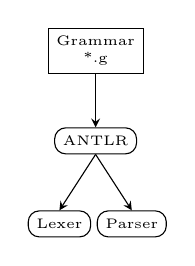
\begin{tikzpicture}[>=stealth, font=\tiny]
    \tikzstyle{edge from parent}=[draw,->]

    \Tree[.\node[language](parser_g){Grammar \\ *.g};
      [.\node[compiler](antlr){ANTLR};
        [.\node[compiler](lexer){Lexer};]
        [.\node[compiler](parser){Parser};]
      ]
    ]
  \end{tikzpicture}
  \caption{ANTLR Parser/Lexer generation}
  \label{fig:antlr_parser_lexer}
\end{figure}

The output of the parser generated by ANTLR is a Parse Tree. ANTLR
also allows specifying a tree transformation to apply to this Parse
Tree. This can be used to automatically generate an Abstract Syntax
Tree (AST).

ANTLR can also generate a tree parser/walker that visit each node of
the AST and applies a certain operation or produces a certain
output. The generation of such a walker is illustrated in Figure
\ref{fig:antlr_tree_walker}.

\begin{figure}[hb!]
  \centering
  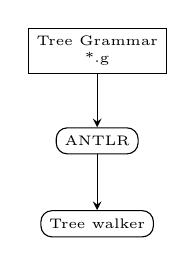
\begin{tikzpicture}[>=stealth, font=\tiny]
    \tikzstyle{edge from parent}=[draw,->]

    \Tree[.\node[language](parser_g){Tree Grammar \\ *.g};
      [.\node[compiler](antlr){ANTLR};
        [.\node[compiler](lexer){Tree walker};]
      ]
    ]
  \end{tikzpicture}
  \caption{ANTLR Tree walker generation}
  \label{fig:antlr_tree_walker}
\end{figure}

\subsection{LLVM}

LLVM\footnote{http://llvm.org} is a compiler framework designed to
support transparent, life-long program analysis and transformation for
arbitrary programs, by providing high-level information to compiler
transformations at compile-time, link-time, run-time, and in idle time
between runs \cite{LLVM:CGO04}.

Traditional compilers were tailored for only a few languages (with the
exception of GCC). However, all traditional compilers suffer from the
large inter-dependency of the basic blocks (Front-end, Optimizer,
Back-end). LLVM tries to solve this by providing an intermediate form
called the LLVM IR. A typical flow involving the basic blocks is
depicted in Figure \ref{fig:llvm_flow}.

\begin{figure}[hb!]
  \centering
   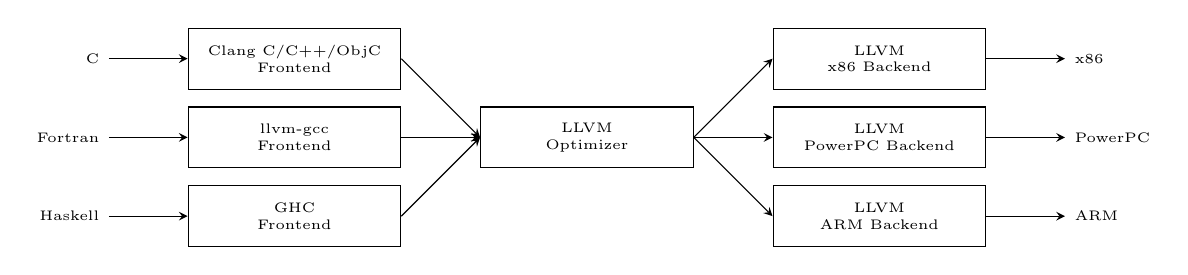
\begin{tikzpicture}[>=stealth]
    \tikzstyle{lang}=[rectangle,draw=black,thin,font=\tiny,inner
    sep=0pt, align=center,minimum width=2.7cm,minimum height=2.2em]

    \tikzstyle{txt}=[font=\tiny]

    \node[lang](llvm_opt){LLVM \\ Optimizer};
    \node[lang](ppc_back)[right=1 cm of llvm_opt]{LLVM \\ PowerPC Backend};
    \node[txt](ppc)[right=of ppc_back]{PowerPC};
    \node[lang](x86_back)[above of=ppc_back]{LLVM \\ x86 Backend};
    \node[txt](x86)[right=of x86_back]{x86};
    \node[lang](arm_back)[below of=ppc_back]{LLVM \\ ARM Backend};
    \node[txt](arm)[right=of arm_back]{ARM};

    \node[lang](gcc_front)[left=1 cm of llvm_opt]{llvm-gcc \\ Frontend};
    \node[txt](fortran)[left=of gcc_front]{Fortran};
    \node[lang](clang_front)[above of=gcc_front]{Clang C/C++/ObjC \\ Frontend};
    \node[txt](c)[left=of clang_front]{C};
    \node[lang](ghc_front)[below of=gcc_front]{GHC \\ Frontend};
    \node[txt](haskell)[left=of ghc_front]{Haskell};

    \draw[->] (clang_front.east) -- (llvm_opt.west);
    \draw[->] (gcc_front.east) -- (llvm_opt.west);
    \draw[->] (ghc_front.east) -- (llvm_opt.west);

    \draw[->] (llvm_opt.east) -- (x86_back.west);
    \draw[->] (llvm_opt.east) -- (ppc_back.west);
    \draw[->] (llvm_opt.east) -- (arm_back.west);

    \draw[->] (x86_back) -- (x86);
    \draw[->] (ppc_back) -- (ppc);
    \draw[->] (arm_back) -- (arm);

    \draw[->] (c) -- (clang_front);
    \draw[->] (fortran) -- (gcc_front);
    \draw[->] (haskell) -- (ghc_front);
  \end{tikzpicture}
  \caption{LLVM typical workflow \cite{llvm_general}}
  \label{fig:llvm_flow}
\end{figure}

Due to its modularity, LLVM has recently seen increased usage in a number
of independent fields:
\begin{itemize}
\item implementing a C/C++ compiler (Clang)
\item implementing C-to-HDL translation
\item implementing a Haskell compiler (GHC)
\item implementing Secure Virtual Architectures (SVA)
\item implementing dynamic translation
\item implementing OpenGL drivers (Mac OS X)
\item implementing OpenCL drivers (AMD)
\end{itemize}

\subsubsection{LLVM IR}

The LLVM IR is the intermediate representation language of the LLVM
project. On its own it is a first-class language with well defined
semantics \cite{llvm_general, llvm_master_thesis}. Variables are in the SSA (Static Single
Assignment) form meaning that they can be only assigned once and they
keep that value for their entire lifetime. All the values residing in
memory need to be loaded to a variable first and stored back to memory
if they wish to be saved. Instructions operate solely upon
variables. In this respect, the LLVM IR resembles the assembly
language of an infinitely many registers Load-Store based RISC
processor.

\begin{lstlisting}[language=C]
unsigned add1(unsigned a, unsigned b) {
  return a+b;
}

// Perhaps not the most efficient way to add two numbers.
unsigned add2(unsigned a, unsigned b) {
  if (a == 0) return b;
  return add2(a-1, b+1);
}
\end{lstlisting}

\begin{lstlisting}
define i32 @add1(i32 %a, i32 %b) {
entry:
  %tmp1 = add i32 %a, %b
  ret i32 %tmp1
}

define i32 @add2(i32 %a, i32 %b) {
entry:
  %tmp1 = icmp eq i32 %a, 0
  br i1 %tmp1, label %done, label %recurse

recurse:
  %tmp2 = sub i32 %a, 1
  %tmp3 = add i32 %b, 1
  %tmp4 = call i32 @add2(i32 %tmp2, i32 %tmp3)
  ret i32 %tmp4

done:
  ret i32 %b
}
\end{lstlisting}

The central concept in constructing LLVM IR is the Module. Each module
consists of functions, global variables and symbol table entries.
Modules can be combined using the LLVM linker \cite{llvm_ir}.

\subsection{GEZEL}

GEZEL is a cycle-accurate hardware description language (HDL) using the
Finite-State-Machine + Datapath (FSMD) model \cite{gezel}.

The basic element is a Signal Flow Graph. It groups operations that
are to be executed concurrently in the same clock cycle.
\begin{lstlisting}[language=GEZEL]
sfg increment {
  a = a + 1;
}
\end{lstlisting}
One or more of these SFGs are used to form a datapath which is the
main building block. It is the smallest GEZEL unit that can stand on
its own and be simulated \cite{gezel}. A datapath can be thought of as
a \emph{module} in Verilog or an \emph{entity} in VHDL. Here is a
full contained example of a counter in GEZEL:
\begin{lstlisting}[language=GEZEL]
dp counter(out value : ns(2)) {
   reg c : ns(2);
   always {
     value = c;
     c = c + 1;
     $display("Cycle ", $cycle, ": counter = ", value);
   }
}

system S {
  counter;
}
\end{lstlisting}

Figure \ref{fig:gezel_workflow} shows how the GEZEL language
can be used as an input to:
\begin{itemize}
\item fdlvhd - a generator that can generate synthesizeable VHDL or
  Verilog
\item fdlsim - a cycle accurate simulator used to verify and validate
  the design
\item gplatform - a co-simulation tool used for HW/SW co-design purposes
\end{itemize}

\begin{figure}[hb!]
  \centering
  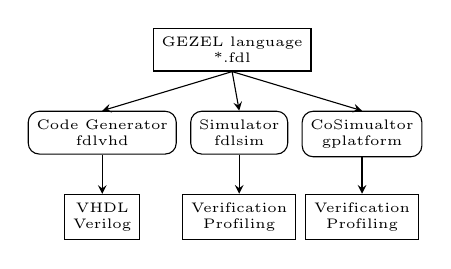
\begin{tikzpicture}[>=stealth, font=\tiny]
    \tikzstyle{edge from parent}=[draw,->]

    \Tree[.\node[language](fdl){GEZEL language \\ *.fdl};
      [.\node[compiler](fdlvhd){Code Generator \\ fdlvhd};
        [.\node[language](vhdl){VHDL \\ Verilog};]
      ]
      [.\node[compiler](fdlsim){Simulator \\ fdlsim};
        [.\node[language](sim){Verification \\ Profiling};]
      ]
      [.\node[compiler](gplatform){CoSimualtor \\ gplatform};
        [.\node[language](cosim){Verification \\ Profiling};]
      ]
    ]
  \end{tikzpicture}
  \caption{GEZEL workflow \cite{gezel}}
  \label{fig:gezel_workflow}
\end{figure}

The co-simulation tool allows to cosimulate GEZEL designs with
instruction-set simulations \cite{gezel}. Supported processors are
ARM, AVR, 8051, MicroBlaze and PicoBlaze. The cosimulation tool allows
for designing a processor-coprocessor pair for a general purpose
processor and a custom dedicated coprocessor.

%%% Local Variables:
%%% TeX-PDF-mode: t
%%% TeX-master: "thesis"
%%% End:


\chapter{Custom framework}

\section{Motivation}

The C code generated by CACE uses GNU GMP which is a multi-precision
arithmetic library. This library is tailored for desktop computers
and is not well suited for small embedded devices. The ZKPDL library
is an interpreter library which is also not well suited for small
embedded devices.

The custom framework build withing the course of this thesis will
attempt to combine the advantages from both projects. As the CACE
project is deemed more suited for the task, the custom framework
will extend CACE. The custom framework will aim to be a compiler
that can produce:
\begin{itemize}
\item Interpreted code
\item JIT (Just In Time) compiled code
\item Compiled code
\end{itemize}

LLVM was chosen as the compiler infrastructure. Its intermediate
form (LLVM IR) is of SSA (Static Single Assignment) form which
allows easy extraction of DFG (Data Flow Graph). This allows
for more aggressive optimization as well as conversion directly
to HDL (Hardware Description Language).

\filbreak

\section{Extensions to GEZEL}

A modification to GEZEL was needed to allow interactivity. A terminal
ipblock was made during the course of this thesis. This ipblock allows
connecting to the host via pseudo-terminals or to other devices via
serial ports.

The ipblock terminal is based on POSIX termios functionality so this
limits the simulator availability to POSIX systems.

\section{Extensions to CACE}

Extensions to the CACE frameworks are presented in Figure
\ref{fig:custom_framework_workflow}. 
The custom part is
further explained in Figure \ref{fig:custom_llvm_workflow}.

\begin{figure}[hbt!]
  \centering
    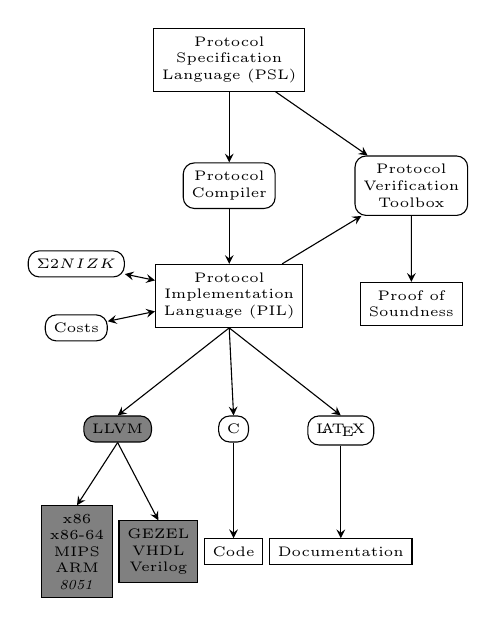
\begin{tikzpicture}[>=stealth,level distance=1.5cm, font=\tiny]
    \tikzstyle{edge from parent}=[draw,->]
    \tikzset{every leaf node/.style={anchor=center}}

    \Tree [.\node[language](psl){Protocol \\ Specification \\ Language (PSL)};
      [.\node[compiler](pc){Protocol \\ Compiler};
        [.\node[language](pil){Protocol \\ Implementation \\ Language (PIL)};
          [.\node[compiler,added](llvm){LLVM};
            \node[language,added](asm){x86 \\ x86-64 \\ MIPS \\ARM \\ \emph{8051}};
            \node[language,added](gezel){GEZEL \\ VHDL \\ Verilog};
          ]
          [.\node[compiler](c){C}; \node[language](code){Code};]
          [.\node[compiler](latex){\LaTeX}; \node[language](doc){Documentation};]
        ]
      ]
    ]

    \node[compiler] (pvt)         [right=of pc,anchor=west]          {Protocol \\ Verification \\ Toolbox}
    child {node[language] {Proof of \\ Soundness}};

    \node[compiler] (sigma) [left=of pil.north west,anchor=center] {$\Sigma 2 N I Z K$};
    \node[compiler] (cost) [left=of pil.south west,anchor=center] {Costs};

    \draw[<->] (sigma) -- (pil);
    \draw[<->] (cost) -- (pil);

    \draw[->] (psl) -- (pvt);
    \draw[->] (pil) -- (pvt);
  \end{tikzpicture}
  \caption{Custom framework (extensions to CACE highlighted)}
  \label{fig:custom_framework_workflow}
\end{figure}

\begin{figure}[hbt!]
  \centering
  \begin{tikzpicture}[>=stealth]
    \tikzstyle{lang}=[rectangle,draw=black,thin,font=\tiny,inner
    sep=0pt, align=center,minimum width=2.7cm,minimum height=2.2em]

    \tikzstyle{txt}=[font=\tiny]

    \node[lang](llvm_opt){LLVM \\ Optimizer};
    \node[lang](ppc_back)[right=1 cm of llvm_opt]{LLVM \\ PowerPC Backend};
    \node[txt](ppc)[right=of ppc_back]{PowerPC};
    \node[lang](x86_back)[above of=ppc_back]{LLVM \\ x86 Backend};
    \node[txt](x86)[right=of x86_back]{x86};
    \node[lang](arm_back)[below of=ppc_back]{LLVM \\ ARM Backend};
    \node[txt](arm)[right=of arm_back]{ARM};
    \node[lang,added](8051_back)[below of=arm_back]{Custom \\ 8051 Backend};
    \node[txt](8051)[right=of 8051_back]{8051};
    \node[lang,added](gezel_back)[below of=8051_back]{Custom \\ GEZEL Backend};
    \node[txt](gezel)[right=of gezel_back]{GEZEL};

    \node[lang,added](pil_front)[left=1 cm of llvm_opt]{PIL \\ Frontend};
    \node[txt](pil)[left=of gcc_front]{PIL};

    \draw[->] (gcc_front.east) -- (llvm_opt.west);

    \draw[->] (llvm_opt.east) -- (x86_back.west);
    \draw[->] (llvm_opt.east) -- (ppc_back.west);
    \draw[->] (llvm_opt.east) -- (arm_back.west);

    \draw[->] (x86_back) -- (x86);
    \draw[->] (ppc_back) -- (ppc);
    \draw[->] (arm_back) -- (arm);

    \draw[->] (pil) -- (pil_front);

    \draw[->] (llvm_opt.east) -- (8051_back.west);
    \draw[->] (llvm_opt.east) -- (gezel_back.west);

    \draw[->] (8051_back) -- (8051);
    \draw[->] (gezel_back) -- (gezel);
  \end{tikzpicture}
  \caption{LLVM custom workflow (changes highlighted)}
  \label{fig:custom_llvm_workflow}
\end{figure}

\newpage

\section{PIL frontend}

PIL frontend flow is depicted in Figure \ref{fig:parser_flow}.  An
input PIL is read by the Lexer producing input for the Parser. The
Parser reads these and generates an abstract syntax tree (AST) which
is fed to the Codegen tree-walker that generates the code (in the form
of LLVM IR). Both the lexer grammar and the parser grammar are
specified in the file pil.g. The tree-walker and the code generator is
specified in the file codegen.g.

\begin{figure}[hbt!]
  \centering
  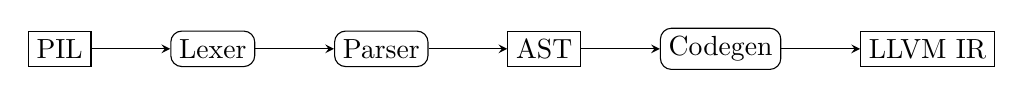
\begin{tikzpicture}[>=stealth]
    \node[language] (pil) {PIL};
    \node[compiler] (lexer) [right=of pil] {Lexer};
    \node[compiler] (parser) [right=of lexer] {Parser};
    \node[language] (ast) [right=of parser] {AST};
    \node[compiler] (codegen) [right=of ast] {Codegen};
    \node[language] (llvm_ir) [right=of codegen] {LLVM IR};

    \draw[->] (pil) -- (lexer);
    \draw[->] (lexer) -- (parser);
    \draw[->] (parser) -- (ast);
    \draw[->] (ast) -- (codegen);
    \draw[->] (codegen) -- (llvm_ir);
  \end{tikzpicture}
  \caption{PIL frontend flow}
  \label{fig:parser_flow}
\end{figure}

\filbreak

The code generation process generates one module per block. The Common
block module is augmented with the functions provided by the VM.
Every other block except the Common block gets a Common block linked
in. This process is depicted in Figure \ref{fig:linker}.

\begin{figure}[hbt!]
  \centering
  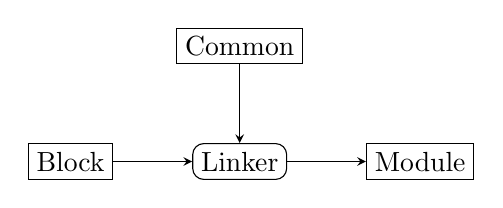
\begin{tikzpicture}[>=stealth]
    \node[language] (block) {Block};
    \node[compiler] (linker) [right=of block] {Linker};
    \node[language] (common) [above=of linker] {Common};
    \node[language] (module) [right=of linker] {Module};

    \draw[->] (block) -- (linker);
    \draw[->] (common) -- (linker);
    \draw[->] (linker) -- (module);
  \end{tikzpicture}
  \caption{Linker}
  \label{fig:linker}
\end{figure}

\section{Coprocessor design}

The coprocessor has:
\begin{itemize}
\item 6 1024-bit registers (u, v, p, R, S, Q)
\item 1 1024-bit datapath (adder and a shifter)
\item 10-bit datapaths and registers for loop and address counters
\end{itemize}

\noindent
The shared memory is used in the following way:
\begin{itemize}
\item 0x600--0x680 1024-bit number
\item 0x680--0x700 1024-bit number
\item 0x700--0x780 1024-bit number
\item 0x780--0x800 command queue (up to 128 commands)
\item 0x800 state signaling from the coprocessor
\end{itemize}

\noindent
The instructions are the following:
\begin{itemize}
\item Halt - stops the execution of the coprocessor and signals the
  done to the main processor
\item Init - initializes the coprocessor (just sets the modulus for now)
\item Montgomery multiplication - executes the Montgomery
  multiplication on the registers u and v and stores the result back
  to u
\item Montgomery squaring - executes the Montgomery squaring of the
  register u and stores the result back to u
\item Montgomery inversion - executes the Montgomery inversion of the
  register u and stores the result back to u (destroys the previous
  values of u and v)
\item Load u from the shared memory - loads the register u from the
  shared memory location 0x00 or 0x80 or 0x100
\item Load v from the shared memory - loads the register v from the
  shared memory location 0x00 or 0x80 or 0x100
\item Store result to shared memory - stores the result of the
  operation to memory location 0x00 or 0x80 or 0x100
\item Store quotient to memory (Montgomery only) - stores the quotient
  of the Montgomery operation to memory location 0x00 or 0x80 or 0x100
\end{itemize}

Special instructions were provided for loading from shared memory
because the coprocessor is 24 times faster with loading from memory
(12 clock cycles for 1 instruction cycle, 2 instruction cycles for
loading on the processor). This way, a third parameter can be stored
in the shared memory for faster fetching.

\subsection{Command queueing}

The idea is to allocate special storage in the shared memory for the
commands the coprocessor should execute. The main processor then
simply fills this memory with the commands the coprocessor needs to
execute. The main processor then starts the coprocessor which will
execute these instructions.

This is also useful if the main processor should be able to perform
other operations while the coprocessor executes the commands
provided. The method has also been tested with the main processor
being slower $144$ (additional $12\textrm{x}$ slowdown) times than the
coprocessor and it gave satisfying results (only $5\textrm{x}$
increase in cycle numbers for RSA).

\subsection{Datapath}

The datapath design revolves around a 1024-bit adder and a shifter in
series. The shifter can shift one position to the left, one position
to the right or just pass the input.

The inputs to the adder are multiplexed between 0, 1, u, v, p, R, S,
power for the x operand. For the v operand, the multiplication step is
multiplexed instead of the power.

The result always gets assigned back to u. This was to allow chaining
of Montgomery multiplications when exponentiation is performed. This
way, no redundant copying is necessary from/to the shared memory. What
is also possible this way is to update the shared memory while the
coprocessor is executing (this helps the elimination of the
communication overhead). The technique was not tested within
this project.

\subsection{Modifications to the Montgomery product}

The Montgomery product computation algorithm has been modified to
include computing the quotient (as is called in
\cite{monpro_doubling}). This allows for doubling the bit-length
(\cite{monpro_doubling, classic_doubling}) of the crypto-coprocessor
in software. This technique was not tested within this project.

\subsection{Software in C}

A library is provided exposing primitives which are executed on the
coprocessor:
\begin{itemize}
\item montpro - Montgomery product
\item montinv - Montgomery inversion
\item modexp - Modular exponentiation
\end{itemize}

\noindent
Also provided are the following software methods:
\begin{itemize}
\item add1024 - adding 1024-bit numbers
\item subtract1024 - subtracting 1024-bit numbers
\item multiply1024 - multiplies 1024-bit numbers to produce a 2048-bit
\item larger\_or\_equal - checks if the number is larger or equal than a number
\end{itemize}

These operations were left in software as they were already fast
enough there. Multiplication was left in case someone would want to
use the bit doubling method. These functions are documented in the
lib.h header file.

\subsection{Hardware in VHDL}

During the co-design phase, separate datapaths were made for the adder
and the bit shifter.  This was to allow a different implementation in
VHDL as the GEZEL-to-VHDL tool (fdlvhd) generates one .vhd file per
datapath. The target devices usually have sophisticated CLA logic
implemented so that efficient adders in terms of space and speed can
be generated.

The same reasoning goes for ASIC design. Usually the libraries
provided from the foundries will include efficient designs of adders
which can be combined to produce the required adder. Even if they
don't, having a separate block allows the designer to concentrate more
on where optimization really counts (critical data path, major effect
on area).

In our specific case, the GEZEL-to-VHDL tool generated 2 1024-bit
adders, one with carry-in and one without it. Manual intervention was
required to change it to a single 1024-bit adder with carry-in. Later
on 2 513-bit adders were used to reduce the slice count even further.
Putting 2 smaller adders helped the synthesis tool spread out and
perform better interconnect.
Custom add\_sub.customxx.vhd are provided in the vhdl subfolder.

%%% Local Variables: 
%%% TeX-PDF-mode: t
%%% TeX-master: "thesis"
%%% End: 


\chapter{Use case: Direct Anonymous Attestation}

%%% Local Variables: 
%%% TeX-PDF-mode: t
%%% TeX-master: "thesis"
%%% End: 


\chapter{Conclusion}

%%% Local Variables: 
%%% TeX-PDF-mode: t
%%% TeX-master: "thesis"
%%% End: 


\printbibliography

\end{document}

%%% Local Variables: 
%%% TeX-PDF-mode: t
%%% TeX-master: t
%%% End: 
